\documentclass[10pt,a4paper]{article}
\usepackage[margin=20mm]{geometry}
\usepackage[T1]{fontenc}
\usepackage{lmodern,graphicx,booktabs,microtype}
\usepackage[hidelinks]{hyperref}
\usepackage{caption}
\captionsetup{font=small,labelfont=bf}
\graphicspath{{../../artifacts/oversight_simulation/figures/}}
\setlength{\parindent}{0pt}\setlength{\parskip}{5pt}
\begin{document}
\begin{center}\Large Computational oversight: accounting and examples\\
\normalsize Supplement to the separate simulation draft\end{center}
All reviewer outcomes and phase times below are \textbf{simulated}. Inputs are the
six reused financial-report contexts and actual saved LLM drafts. No human
observations, questionnaires or participant identifiers were generated.

\begin{figure}[h!]
\centering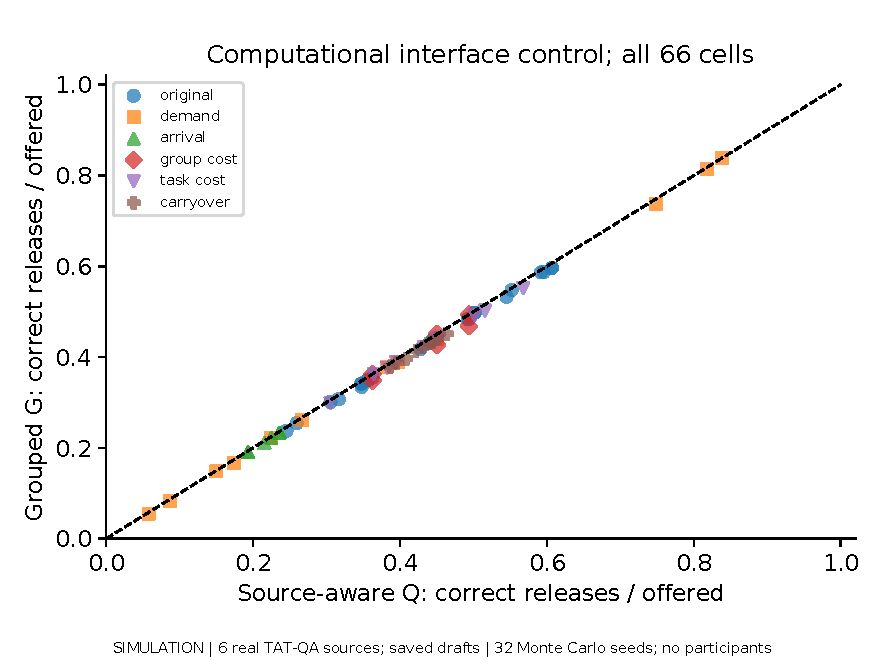
\includegraphics[width=.75\linewidth]{source_aware_control.pdf}
\caption{All 66 declared parameter-cell means. The diagonal is equal correct
release fraction. No grouped mean exceeds the identically source-aware queue.
Points reuse sources and parameter settings; they are not independent people or
reports. Zero-overhead equality is structural.}
\end{figure}
\begin{figure}[h!]
\centering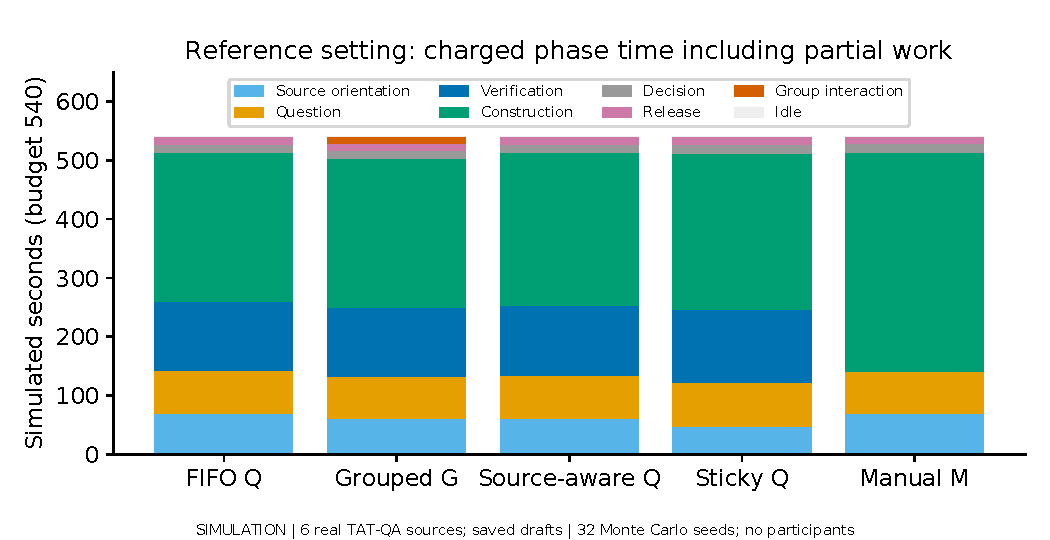
\includegraphics[width=.89\linewidth]{time_decomposition.pdf}
\caption{Assigned review phases in the original nine-minute reference setting.
Partial last reviews consume time through cutoff. Components plus idle sum to
540 seconds. These are model components, not observed reading or attention time;
the completed question subsets can differ.}
\end{figure}

\clearpage
\section*{First qualifying positive and adverse traces}
Selection is by declared configuration order, then packet rotation, then seed.
The traces were not chosen by effect magnitude. Each source label is an actual
context identity; black ticks are constructed arrivals. Colors identify a review
attempt that releases a correct or incorrect answer. An unreleased or deferred
attempt remains gray even if a later attempt releases its question.

\begin{figure}[h!]
\centering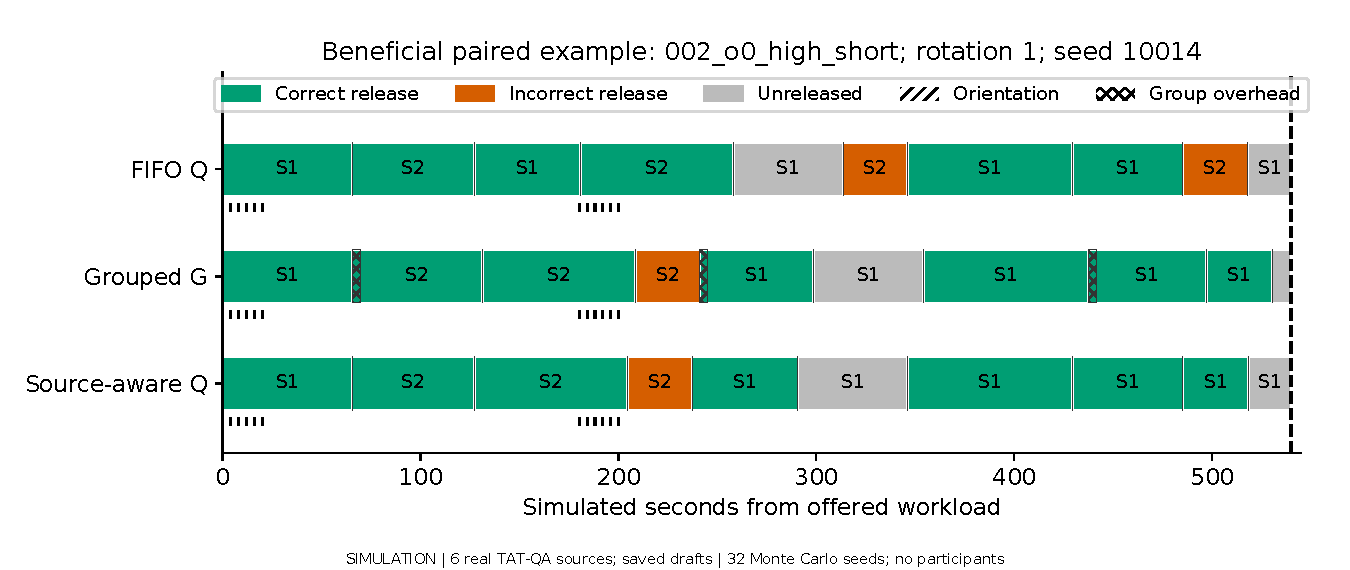
\includegraphics[width=\linewidth]{timeline_beneficial.pdf}
\caption{First individual run with more correct releases in G than FIFO Q.
Orientation cost is zero. G releases one more correct answer, despite extra group
overhead. The difference is which potential outcomes reach cutoff, not a saving
in context reconstruction. This setting's cell mean actually favors FIFO.}
\end{figure}
\begin{figure}[h!]
\centering
\includegraphics[width=\linewidth]{timeline_unfavorable.pdf}
\caption{First adverse paired run. With zero orientation cost and ideal review,
group overhead leaves a correct answer unreleased at cutoff that both queues
release. Source grouping preserves the request but does not complete it. All
subsequent approvals and repairs are simulated, not actual model continuations.}
\end{figure}
The positive example has nine common attempted question/attempt pairs, zero
planned orientation saving and 12 seconds of additional grouping interaction.
The adverse example has seven common pairs, zero orientation saving and eight
seconds of group interaction. These balances do not equate different final
subsets. A favorable single trace cannot establish a beneficial operating region.

Original questions, draft fields, source IDs and corresponding simulation-run
identifiers are retained in \path{research/oversight_simulation/EXAMPLES.md}.
The selected tied trace is also retained there. Full command traces permit
inspection of decisions and output versions; no reference annotation is exposed
to the selector.
\end{document}
